\chapter{Разработка нового алгоритма построения выпуклой оболочки} \label{chapt2}

\section{Формализация понятия выпуклой оболочки} \label{sect2_1}

Формализация задачи "--- это очень важная часть любого исследования, которая позволяет правильно анализировать результаты работы. Итак, чтобы разработать алгоритм построения выпуклой оболочки конечного множества точек на плоскости, необходимо формализовать данное понятие.

Пусть дано множество $S$ точек. Выпуклой оболочкой данного множества называется наименьшее выпуклое множество, содержащее $S$. Формально выпуклая оболочка может быть определена как пересечение всех выпуклых множеств, которые содержат $S$.

Это определение является самым популярным и общим, но оно слишком далеко от практики, поэтому мы будем использовать другое. Заметим, что разрабатываемый алгоритм должен работать только для плоскости, поэтому мы будем использовать определение, которое работает только для случая двумерного пространства.

Для формализации понятия выпуклой оболочки, нам снова понадобится предикат $ccw$, описанный в формуле \eqref{eq:ccw}. Выпуклой оболочкой множества $S$ будет называться выпуклый многоугольник $T$ с вершинами $t_i \in S$, пронумерованными против часовой стрелки для $i = 1,...,n$~\cite{pichardie2001formalizing}. Причём обязательно выполнения условия \eqref{eq:convex_hull_def}.

\begin{equation}\label{eq:convex_hull_def}
\forall [t_i, t_{i+1}] \in T, p \in S \backslash \{ t_i, t_{i+1} \} : ccw(t_i, t_{i+1}, p)
\end{equation}

Это выражение утверждает, что каждая точка $p$, принадлежащая $S$, кроме текущего ребра $t_i, t_{i+1}]$, находится слева от него. Это свойство выпуклой оболочки отлично показано на рисунке \ref{img:convex_hull_def} с помощью ориентированных рёбер. Видно, точек справа от ребра нет, иначе бы это ребро не принадлежало выпуклой оболочке.

\begin{figure}[hbt]
	{\centering
		\hfill
		\subbottom[Конечное множество точек $S$\label{img:convex_hull_def_1}]{%
			\includesvg[width=0.45\linewidth]{convex_hull_def_1}}
		\hfill
		\subbottom[Выпуклая оболочка с ориентированными рёбрами\label{img:convex_hull_def_2}]{%
			\includesvg[width=0.45\linewidth]{convex_hull_def_2}}
		\hfill
	}
	\caption{Формализация понятия выпуклой оболочки}
	\label{img:convex_hull_def}
\end{figure}

Заметим, что это определение никак не нарушает требование минимальности выбранного многоугольника, так как мы составляем выпуклую оболочку из точек, которые принадлежат множеству $S$.

\section{Описание алгоритма основанного на использовании бинарного дерева} \label{sect2_2}

\subsection{Основная идея} \label{subsect2_2_1}

Основная идея предлагаемого в данной работе алгоритма очень похожа на принцип, лежащий в основе инкрементального алгоритма, уже рассмотренного выше. Мы можем хранить точки в сбалансированном по высоте двоичном дереве поиска. Точки в инкрементальном алгоритме хранились в верхнем и нижнем деревьях и были отсортированы по координате $x$. Мы будем использовать другой подход, который позволит хранить точки только в одном дереве, узлы (точки) будут отсортированы по углу относительно приблизительного центра выпуклой оболочки.

Чтобы объяснить работу алгоритма нам понадобится уже известный нам предикат $ccw$, определённый в формуле \eqref{eq:ccw} и понятие экстремальной точки.

Экстремальная точка множества $S$ "--- это точка, которая точно принадлежит выпуклой оболочке $S$. Обычно это точка, которая лежит дальше от всех по какому либо параметру. Например, самая левая или верхняя точка точно будет входить в итоговую выпуклую оболочку.

Пусть дано множество точек $S$ и необходимо найти выпуклую оболочку данного множества.

Первый шаг алгоритма "--- это нахождение приближенного центра, с помощью которого будут отсортированы в дереве точки. Хорошей аппроксимацией центра для наших целей будет среднее арифметическое трёх экстремальных точек:
\begin{itemize}
	\item левая крайняя точка $A$;
	\item правая крайняя точка $B$;
	\item точка $C$, которая наиболее удалена от линии $A,B$.
\end{itemize}

На рисунке~\ref{img:my_extreme_points_1} показан пример, найденных на первом шаге алгоритма, экстремальных точек. Потом на рисунке~\ref{img:my_extreme_points_2} находится точка $D$ "--- это приближённый центр выпуклой оболочки, который мы искали. После нахождения центра мы добавляем точки $A, B, C$ в наше дерево поиска.

\begin{figure}[hbt]
	{\centering
		\hfill
		\subbottom[\label{img:my_extreme_points_1}]{%
			\includesvg[width=0.45\linewidth]{my_extreme_points_1}}
		\hfill
		\subbottom[\label{img:my_extreme_points_2}]{%
			\includesvg[width=0.45\linewidth]{my_extreme_points_2}}
		\hfill
	}
	\caption{Нахождение приближённого центра выпуклой оболочки}
	\label{img:my_extreme_points}
\end{figure}

Остальные точки будут добавлены в случайном порядке. Рассмотрим процесс добавления очередной точки в текущую выпуклую оболочку множества.

Пусть мы уже построили дерево поиска, в котором содержится наша выпуклая оболочка, отсортированная по углу относительно центра $D$, найденного ранее. Теперь необходимо добавить новую точку $A$.

Первое, что необходимо найти "--- это две точки $L$ и $R$. Точки $L$, $R$ "--- это точки слева и справа соответственно от $A$ по углу относительно центра $D$. Как видно на рисунке \ref{img:my_find_lr}, все точки хранятся по углу относительно точки $D$, и поэтому поиск точек не вызывает труда.

\begin{figure}[hbt]
	\centering
	\includesvg[width=\linewidth]{my_find_lr}
	\caption{Нахождение точек $L, R$ в бинарном дереве поиска}
	\label{img:my_find_lr}
\end{figure}

Заметим, что может так оказаться, что точки $L$ и $R$ окажутся в противоположных частях бинарного дерева поиска. Это показано на рисунке \ref{img:my_find_cyclic}. Поэтому мы будем считать, что наше используемое сбалансированное двоичное дерево поиска является цикличным. Заметим, что для этого не требуется никаких специальных дополнительных структур данных. Всё, что нужно делать "--- это при обходе дерева и достижении последней точки, переходить на первую.

\begin{figure}[hbt]
	\centering
	\includesvg[width=\linewidth]{my_find_cyclic}
	\caption{Демонстрация цикличности используемого дерева поиска}
	\label{img:my_find_cyclic}
\end{figure}

После чего может быть 2 случая. Если $ccw(L, R, A)$ не выполняется, то новая точка $A$ не должна быть частью выпуклой оболочки и может быть пропущена. Этот случай показан на рисунке~\ref{img:my_point_cases_1}. Иначе $A$ должна быть частью выпуклой оболочки и мы продолжим добавлять её. Это показано на рисунке~\ref{img:my_point_cases_2}.

\begin{figure}[hbt]
	{\centering
		\hfill
		\subbottom[\label{img:my_point_cases_1}]{%
			\includesvg[width=0.49\linewidth]{my_add_point_1}}
		\hfill
		\subbottom[\label{img:my_point_cases_2}]{%
			\includesvg[width=0.49\linewidth]{my_add_point_2}}
		\hfill
	}
	\caption{Добавление новой точки в выпуклую оболочку}
	\label{img:my_point_cases}
\end{figure}

Итак, мы определили, что точка $A$ должна быть на выпуклой оболочке. Теперь необходимо удалить точки, которые будут внутри оболочки после добавления точки $A$. Это делается с помощью итерации по точкам вправо (аналогичный алгоритм должен быть выполнен для левой стороны) от новой точки. Чтобы определить должна ли точка быть удалена или нет мы будем использовать подход, похожий на тот, который используется в алгоритме Грэхема. Каждые два смежных ребра выпуклой оболочки должны лежать против часовой стрелки.

Пусть следующая точка, которая рассматривается на удаление "--- это $B$. Рассмотрим процесс удаления точки $B$.
\begin{enumerate}
	\item Назовем точку, которая идет следующей после $B$, $C$.
	\item Если $ccw(C, B, A)$ тогда $B$ не должна быть удалена и мы должны прекратить удаление точек в эту сторону, потому что все точки после $B$ уже удовлетворяют условию выпуклой оболочки. По сути этот предикат и проверяет условие лежания смежных ребер против часовой стрелки, о котором говорилось ранее.
	\item Иначе точка $B$ должны быть удалена, так как она оказалась внутри новой выпуклой оболочки.
	\item После чего необходимо рассмотреть точку $C$ как следующего кандидата на удаление и перейти к шагу 1.
\end{enumerate}

На рисунках \ref{img:my_points_deletion_1_1} и \ref{img:my_points_deletion_1_2} можно видеть, что точки $C, B, A$ лежат по часовой стрелке, поэтому точка $B$ должна быть удалена из выпуклой оболочки. Рисунок \ref{img:my_points_deletion_2_1} демонстрирует, что мы должна прекратить удаление точек справа от новой точки, так как $C, B, A$ теперь формирует тройку, которая лежит против часовой стрелки. Аналогично удаление не нужно производить слева от точки, что показано на рисунке \ref{img:my_points_deletion_2_2}. Действительно, на рисунках видно, что в конце получилась готовая выпуклая оболочка добавленных на текущий момент точек.

\begin{figure}[hbt]
	{\centering
		\hfill
		\subbottom[\label{img:my_points_deletion_1_1}]{%
			\includesvg[width=0.49\linewidth]{my_add_point_3}}
		\hfill
		\subbottom[\label{img:my_points_deletion_1_2}]{%
			\includesvg[width=0.49\linewidth]{my_add_point_4}}
		\hfill
	}
	\caption{Удаление точек, которые оказались внутри выпуклой оболочки}
	\label{img:my_points_deletion_1}
\end{figure}

\begin{figure}[hbt]
	{\centering
		\hfill
		\subbottom[\label{img:my_points_deletion_2_1}]{%
			\includesvg[width=0.49\linewidth]{my_add_point_5}}
		\hfill
		\subbottom[\label{img:my_points_deletion_2_2}]{%
			\includesvg[width=0.49\linewidth]{my_add_point_6}}
		\hfill
	}
	\caption{Критерий завершения удаления точек}
	\label{img:my_points_deletion_2}
\end{figure}

Как видно этот процесс очень схож с процессом добавления точек в инкрементальном алгоритме. Существуют такие небольшие различия, как одно дерево вместо двух, цикличность этого дерева, отсутствие граничного случая на стыке двух деревьев и т.д. Они хоть и небольшие, но позволяют алгоритму быстрее добавлять точки в выпуклую оболочку.

Блок-схема всего алгоритма показана на рисунках \ref{img:my_algo} и \ref{img:my_algo_deletion}.

\begin{figure}
	\centering
	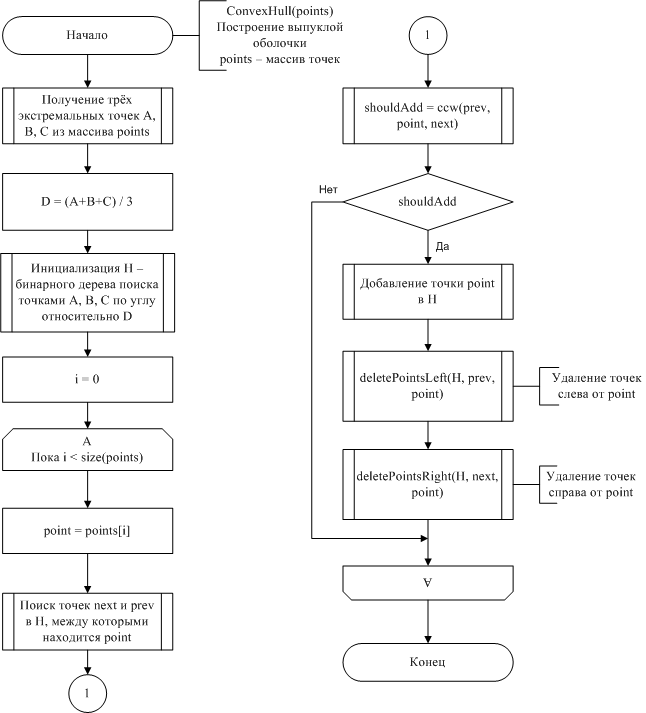
\includegraphics[width=\linewidth]{my_algo}
	\caption{Блок-схема работы предлагаемого алгоритма}
	\label{img:my_algo}
\end{figure}

\begin{figure}
	\centering
	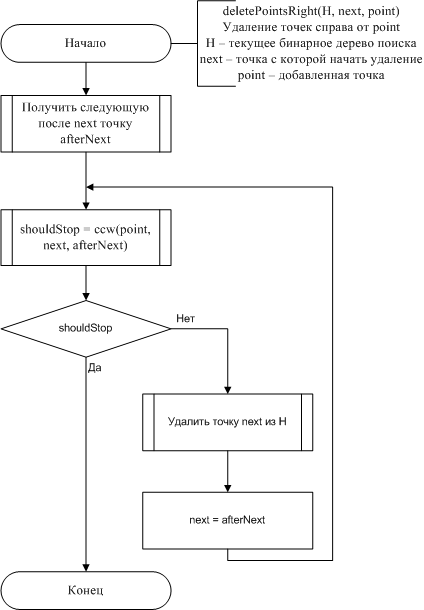
\includegraphics[width=0.7\linewidth]{my_algo_2}
	\caption{Блок-схема функции удаления точек перед добавлением точки point}
	\label{img:my_algo_deletion}
\end{figure}

\subsection{Детали реализации} \label{subsect2_2_2}

Первая важная деталь, которая упрощает реализацию нашего алгоритма "--- это конечно преобразование точек. Намного удобнее считать, что приближённый центр $D$, получение которого описывалось в предыдущей главе "--- это точка $0, 0)$. Как показано в \eqref{eq:ccw} мы вычисляем $ccw$ через $det$, а вычислять $det(A, B, D)$ легче, если $D_x = 0$ и $D_y = 0$. Также нельзя забывать про конечную цель вычисления выпуклой оболочки. Для вычисления дескриптора опять намного удобнее пользоваться координатами уже переведёнными в центр объекта, так как на дескриптор никак не должно влиять положения объекта на изображении.

Вторая деталь, которая также важна при реализации "--- это углы относительно центра, про которые мы так много говорили. Вычисление углов через тригонометрические операции "--- это очень долго, и в этом случае наш алгоритм не смог бы конкурировать по производительности с самыми популярными алгоритмами вычисления выпуклой оболочки.

Необходимо придумать предикат, который бы определял положение точек в дереве, которое хранит текущую выпуклую оболочку. Первой попыткой придумать такой предикат будет использование предиката $ccw$, как это показано в \eqref{eq:my_ccw_predicate}.

\begin{equation}\label{eq:my_ccw_predicate}
A<B=ccw(A, B, (0, 0))
\end{equation}

Заметим, что можно использовать точку $(0, 0)$ как центр, так как точки $A, B$ уже преобразованы в новую систему координат.

К сожалению, такой предикат не соответствует strict weak ordering~\cite{isoCppStd2017}, потому что не выполняется транзитивность. Как можно видеть на рисунке \ref{img:non_transitivity_1} выполняется $ccw(A, B, D)$, поэтому $A$ меньше $B$. При этом выполняется $ccw(B, C, D)$, поэтому $B$ меньше $C$. Но на рисунке \ref{img:non_transitivity_2} в это еже время показано, что не выполняется $ccw(A, C, D)$, то есть $A$ не меньше $C$. В итоге имеем $A < B < C <= A$, что, очевидно, неверно.

\begin{figure}[hbt]
	{\centering
		\hfill
		\subbottom[\label{img:non_transitivity_1}]{%
			\includesvg[width=0.45\linewidth]{non_transitivity_1}}
		\hfill
		\subbottom[\label{img:non_transitivity_2}]{%
			\includesvg[width=0.45\linewidth]{non_transitivity_2}}
		\hfill
	}
	\caption{Нетранзитивный предикат}
	\label{img:non_transitivity}
\end{figure}

Итак, необходимо сделать такую функцию, которая принимает точки $A$ и $B$ и возвращает $true$, если $A$ меньше $B$, иначе $false$. Эта функция будет использована в сбалансированном дереве поиска как компаратор. Был использован следующий алгоритм:

\begin{algorithm}[H]
	\caption{BSTPredicate "--- компаратор для сравнения точек}
	\label{alg:bst_predicate}
	\begin{algorithmic}[1]
		\Procedure{BSTPredicate}{$A, B$}
		\State $leftUp \gets 0<y_A$
		\State $rightUp \gets 0<y_B$
		\If {$leftUp \neq rightUp$}
			\Return $leftUp < rightUp$
		\EndIf
		\If {$(y_A=0) \& (y_B=0)$}
			\Return $(0<x_A) < (0<x_B)$
		\EndIf
		\Return $ccw(A, B, (0, 0))$
		\EndProcedure
	\end{algorithmic}
\end{algorithm}

Эта несложная функция реализует корректный для сортировки предикат. Для этого изначально она делит всю плоскость координат на две части: верхнюю и нижнюю. Как мы видим предикат принимает 2 точки $A$ и $B$. Рассмотрим три случая:
\begin{enumerate}
	\item Если эти точки лежат на разных сторонах. Например, точка $A$ лежит ниже точки $B$, тогда предикат вернет $true$, что будет означать, что $A$ меньше $B$.
	\item Граничный случай, когда обе точки находятся на оси $x$. Тогда нужно определить с какой стороны от оси $y$ они находятся. Если с одной, то токи равны, потому что угол до них одинаков. Иначе меньше точка, которая находится слева.
	\item Если точки находятся в одной полуплоскости, то предикат $ccw$, показанный в формуле \eqref{eq:ccw}, отлично справляется со своей задачей.
\end{enumerate}

Пример порядка точек, вычисленного, с помощью алгоритма BSTPredicate показан на рисунке \ref{img:BSTPred_ordering}.

\begin{figure}[hbt]
	\centering
	\includesvg{BSTPred_ordering}
	\caption{Сортировка точек предикатом BSTPredicate}
	\label{img:BSTPred_ordering}
\end{figure}

\section{Доказательство корректности работы алгоритма} \label{subsect2_3}

Доказательство корректности работы алгоритма удобнее всего построить с помощью математической индукции.

Базис индукции "--- это 3 изначально добавленные в выпуклую оболочку точки. Необходимо доказать, что в начальном шаге выпуклая оболочка удовлетворяет условию \eqref{eq:convex_hull_def}.

Любые 3 точки, не лежащие на одной прямой, являются выпуклой оболочкой, так как они формируют треугольник. Единственное условие, которое необходимо соблюсти "--- это правильный порядок этих точек. Это условие обеспечивается бинарным деревом поиска с предикатом BSTPredicate, поэтому первые три точки являются выпуклой оболочкой.

Пусть теперь для $N$ рассмотренных точек была построена валидная выпуклая оболочка и сейчас рассматривается точка $p_{N+1}$. Как описано выше, при добавление точки необходимо рассматривать два варианта.

Если точка оказалась внутри выпуклой оболочки, то она не может быть добавлена. Заметим, если точка внутри выпуклого многоугольника, то она находится справа от любого его ребра. Этот случай уже был показан на рисунке \ref{img:convex_hull_def_2}. Очевидно, что если точка не добавляется и до этого выпуклая оболочка была правильно построена, то и после она будет валидна.

Второй случай является более сложным. Точка должна быть добавлена в существующую выпуклую оболочку. Процесс удаление точек уже был показан на рисунке \ref{img:my_points_deletion_1}. Важное в этом процессе, что он делается по критерию не выполнения $ccw(C, B, A)$, что абсолютно идентично критерию выпуклой оболочки в формуле \eqref{eq:convex_hull_def}. На рисунке \ref{img:my_proof_1} показано выполнение условия выпуклой оболочки для новой добавленной точки. Из-за условия удаления точно известно, что после добавления новой точки $p_{N+1}$ удалённые точки и точки $C_1, C_2$ находятся слева от новых рёбер $p_{N+1}, A$ и $B, p_{N+1}$. Осталось показать, что остальные точки также лежат левее этих рёбер.

\begin{figure}[hbt]
	\centering
	\includesvg{my_proof_1}
	\caption{Состояние выпуклой оболочки после добавления новой точки}
	\label{img:my_proof_1}
\end{figure}

Предположим, что существует такая точка $k$, что она лежит правее новых ребер. Заметим, что эта точка может лежать только левее прямой $B, A$, так как все точки правее были рассмотрены в процессе удаления. Также заметим, что было показано, что выполняются предикаты $ccw(p_{N+1}, A, C_2)$ и $ccw(C_1, A, p_{N+1})$. В это же время для ребер $A, C_2$ и $C_1, B$ по предположению индукции мы знаем, что все точки лежат левее их. Получаем противоречие, потому что точка $k$ должна лежать правее новых рёбер, но при этом она должна лежать левее линий $C_1, B$; $B, A$; $A, C_2$. На изображении~\ref{img:my_proof_2} отлично видно, что две эти области не пересекаются. Таким образом, корректность выпуклой оболочки после добавления новой точки сохраняется.

\begin{figure}[hbt]
	\centering
	\includesvg{my_proof_2}
	\caption{Области, где может лежать точка}
	\label{img:my_proof_2}
\end{figure}

\section{Оценка сложности алгоритма} \label{subsect2_4}

Пусть дано множество точек $S$ размера $N$.

Первое, что необходимо определить "--- это временную сложность алгоритма.

На шаге инициализации алгоритма проводиться поиск трёх экстремальных точек. Это делается за $2 N$ шагов, так как надо сначала найти самые левую и правую точки, а потом найти самую дальнюю от них другую точку.

После чего точки рассматриваются в случайном порядке. Изначально необходимо найти положение точки в бинарном дереве. Эта операция делается за $O(\log h)$, где $h$ "--- это текущее количество точек в выпуклой оболочке.

Если эту точку необходимо добавить, то далее удаляются все точки, которые после добавления точки окажутся внутри выпуклой оболочки. Сложность операции удаления точки может варьироваться для разных сбалансированных двоичных деревьев поиска. В стандарте языка C++ сказано, что амортизированная сложность операции удаления из $std::set$ по итератору является $O(1)$~\cite{isoCppStd2017}. Поэтому будем считать, что у операции удаления константная сложность.

Во время работы алгоритма максимальное количество удалений не может превышать $N$, так как всего $N$ точек рассматривается. Поэтому эта операция занимает $O(N)$ времени.

Пусть максимальный размер выпуклой оболочки за время работы алгоритма равен $M$. Тогда сложность поиска точек за всё время работы алгоритма равна $O(N \log M)$.

В итоге сложность алгоритма равна:
\[
O(2 N + N + N \log M) = O(N \log M)
\]

Заметим, что в обычном случае количество точек в дереве будет примерно около $H$ всё время работы алгоритма, что позволяет нам сказать, что средняя сложность будет равняться $O(N \log H)$, где $H$ "--- это количество точек в финальной выпуклой оболочке. Заметим, что так как точки добавляются в случайном порядке, обычно именно такая сложность и будет достигаться. 

Если рассматривать точки не в случайном порядке, то возможно подобрать тесты, при которых сложность алгоритма будет равняться $O(N \log N)$. Поэтому мы считаем, что в худшем случае наш алгоритм будет иметь именно такую временную сложность. 

Сколько памяти потребляет предлагаемый алгоритм? Кроме хранения входных данных предлагаемому в данной работе алгоритму необходимо хранить также сбалансированное двоичное дерево поиска с точками, которые сейчас принадлежат выпуклой оболочке. Поэтому сложность по памяти будет равняться $O(M)$. Аналогично временной сложности средняя равна $O(H)$, когда же в худшем случае это $O(N)$.

\section{Выводы} \label{subsect2_5}

Разработанный в этой главе алгоритм построения выпуклой оболочки имеет множество преимуществ, которые безусловно нужны при выполнении задач компьютерного зрения. Он:
\begin{itemize}
	\item является оптимальным в среднем случае (имеет сложность $O(n \log h)$);
	\item предоставляет дополнительные данные для будущего построения дескриптора (приблизительный центр объекта);
	\item имеет возможность к настройке под конкретные практические нужды с помощью изменения реализации сбалансированного двоичного дерева поиска (AVL, красно-чёрные деревья, и т.д.);
	\item прост в имплементации;
	\item позволяет добавлять точки и после окончания работы алгоритма.
\end{itemize}

Заметим, что требования, которые выдвигались в выводах к первой главе были удовлетворены.

До сих пор обсуждались лишь теоретические выкладки. Следующий шаг "--- это проверка алгоритма на практике.
